\section{Graphs of Tables of Critical Frequencies} \label{Graphs_Tables}

\subsection{Implicational quantifiers}
By the means stated in section \ref{Graphs} we examined the three most used implicational quatifiers: 
\emph{founded implication}, \emph{lower} and \emph{upper critical implication}. Figure \ref{fig:Implicational} displays graphs of maximal b's for $p=0.8$, $\alpha=0.05$ and for $a=0\dots1000$.

\begin{figure}[ht]
\centering
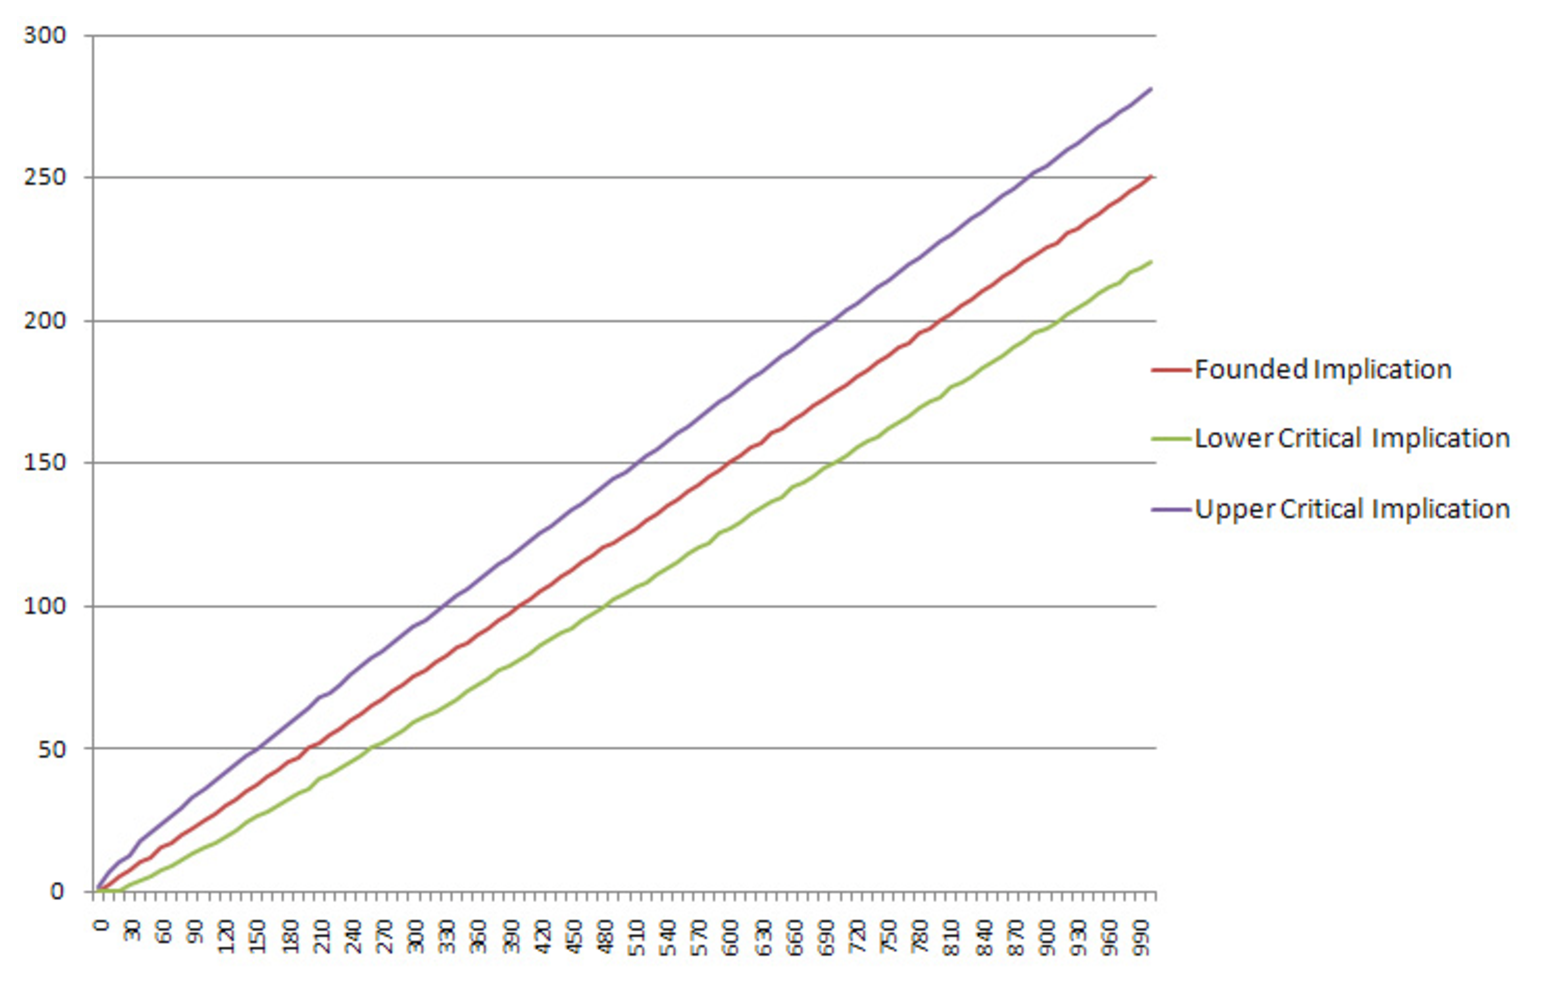
\includegraphics[width=115mm]{Implicational.eps}
%\mbox{\resizebox{125mm}{!}{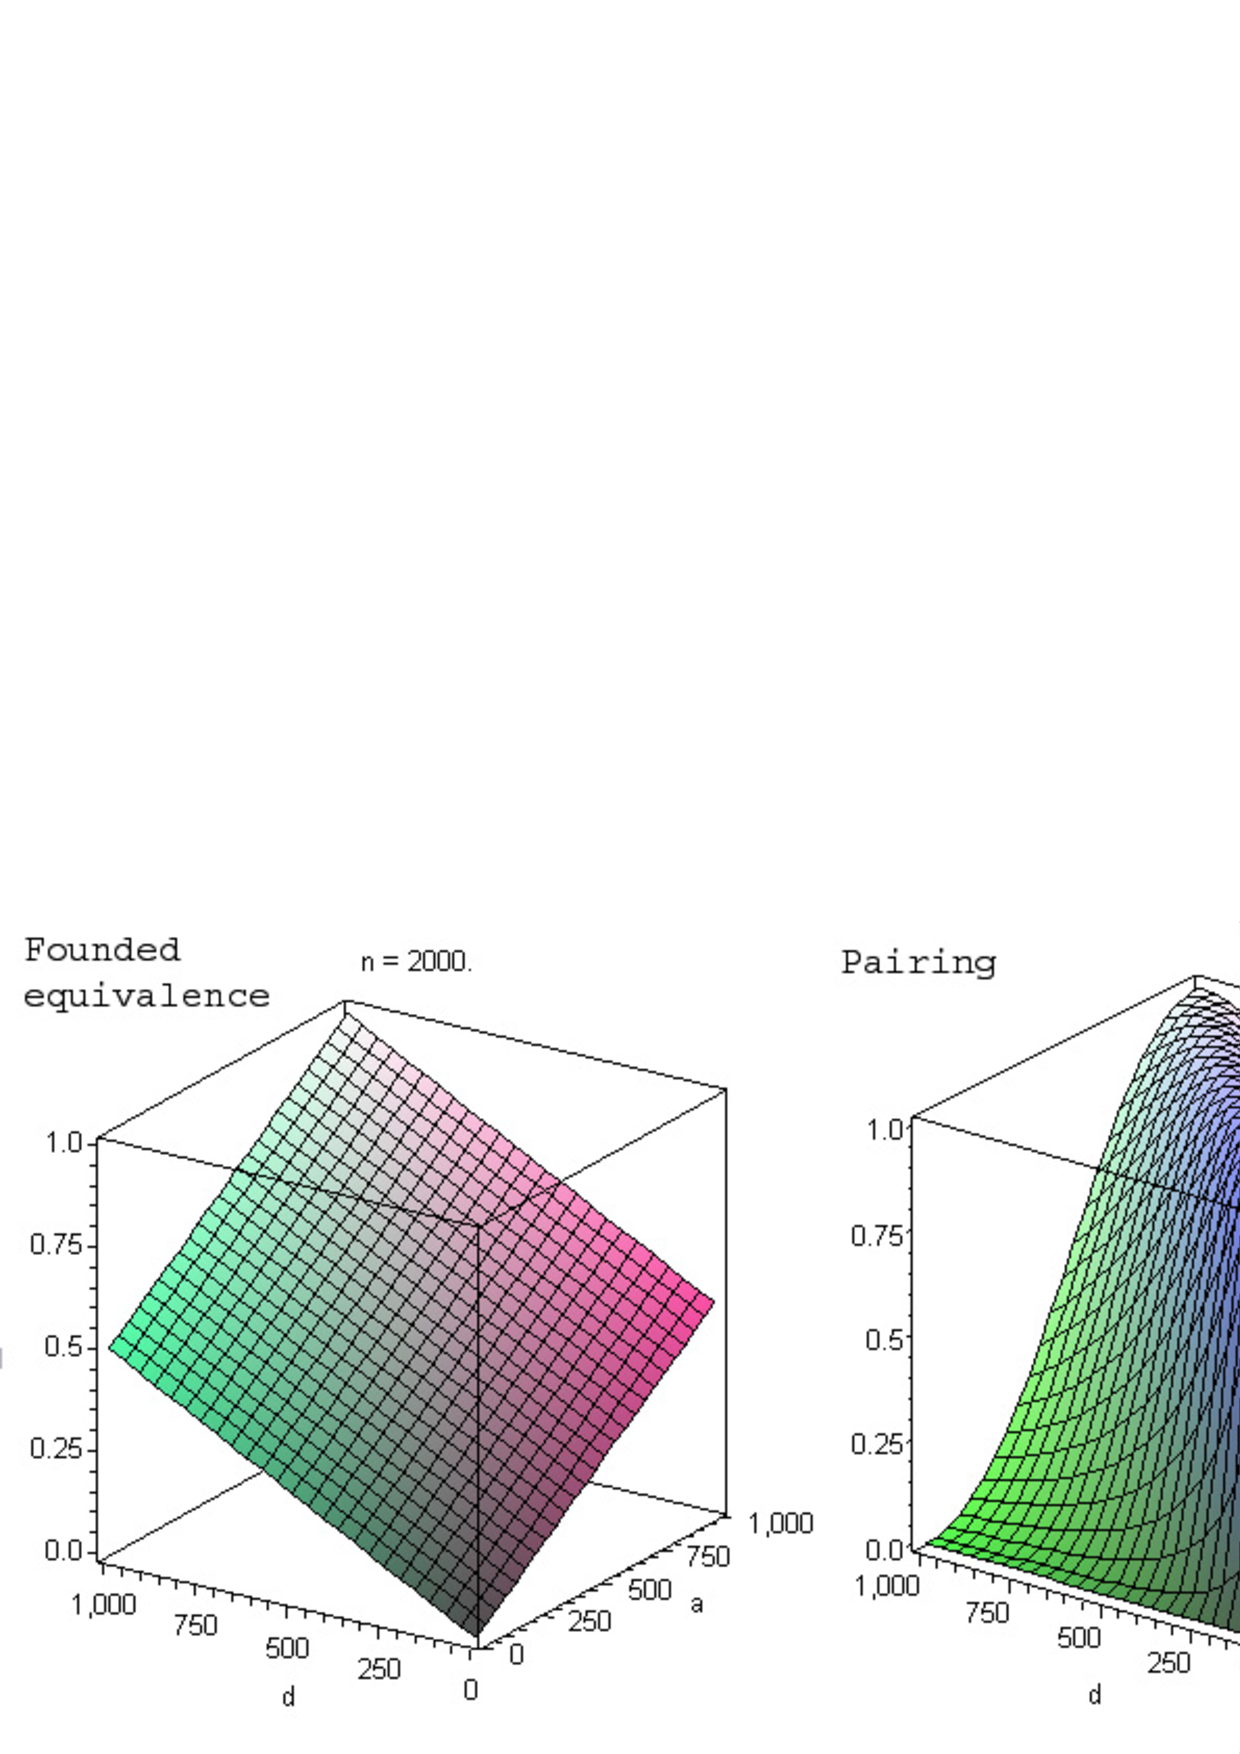
\includegraphics{FE-Pairing.png}}}
\caption{Tables of maximal b's for implicational quantifiers}
\label{fig:Implicational}
\end{figure}

The graph shows, that we cannot use (in the examined range of $a$) computationally simple \emph{founded implication} instead of statistically sound but computationally demanding \emph{lower} and \emph{upper critical implications}. This is an important result that could not be obtained without construction of \emph{tables of maximal b's}.

We can think of \emph{tables of maximal b} as another definition of the quantifier. It is function from $a$ to $b$. For \emph{founded implication} we know exact definition of the function. It is 
%
%
%$f(a) = \frac{a(1-p)}{p}$ 
%
%VERSE RAUCH:
$ Tb_{\Rightarrow_{p}} = \left\lceil \frac{a(1-p)}{p} + 1 \right\rceil$
%
and can be obtained by basic arithmetic operations, $ \left\lceil x \right\rceil$ means upper integer part of $x$. 
To our best knowledge, arithmetic extraction of the function for critical implications is impossible. For construction of the table, we programmed iterations over $a$ and $b$ and checked, when the evaluation function stops being valid. This is computationally demanding because of the factorials in binomial coefficient and cannot be done effectively for very high numbers. Thus the method cannot be used to calculate values of functions close to infinite values.

To get a better idea about the functions, we examined their slopes. It is constant for \emph{founded implication} and equals the $\frac{1-p}{p}$. Slopes of the critical implication in chosen points ($a$ values) are shown in table \ref{tab:slopes}.

\begin{table}[ht]
	\centering
	\caption{Slopes of critical frequencies}	
		\label{tab:slopes}
		\begin{tabular}{|p{4cm}|p{1cm}|p{1cm}|p{1cm}|p{1cm}|p{1cm}|p{1cm}|p{1cm}|}
			\hline
			$p=0.8, \alpha=0.05$
			 &\textbf{10}&\textbf{100}&\textbf{300}&\textbf{500}&\textbf{700}&\textbf{900}&\textbf{1000}\\
			\hline
			\textbf{Lower Critical Impl.}&0.1&0.16&0.2&0.21&0.215&0.22&0.22\\
			\hline
			\textbf{Upper Critical Impl.}&0.7&0.36&0.306&0.294&0.285&0.282&0.281\\
			\hline
		\end{tabular}
\end{table}

The table reveals interesting facts. Note, that the difference between slopes of critical implications and slope of \emph{founded implication} remains the same. This means that the critical implications maximal b's tables are symmetric with respect to the \emph{founded implication} maximal b table. 

Our working hypothesis is, that 
%
%VERSE RAUCH
%
$$\lim_{a\rightarrow\infty} \frac{Tb_{\Rightarrow^{!}_{p, \alpha}}(a)}{a} = \lim_{a\rightarrow\infty} \frac{Tb_{\Rightarrow^{?}_{p, \alpha}}(a)}{a} = \lim_{a\rightarrow\infty} \frac{Tb_{\Rightarrow_{p}}(a)}{a} = %\frac{dTb_{\Rightarrow_{p}}}{da} = 
\frac{1-p}{p} \mbox{ .}$$ 

However we are currently unable to prove it. If we combine the hypothesis with results from figure \ref{fig:Implicational} (for fixed $p, \alpha$ the lower critical implication \emph{is I-stronger than} founded implication, which \emph{is I-stronger than} upper critical implication, than for all natural $a$, 
$Tb_{\Rightarrow^{!}_{p, \alpha}}(a) < Tb_{\Rightarrow_{p}}(a) < Tb_{\Rightarrow^{?}_{p, \alpha}}(a)$.

\subsection{Quantifiers with F-property}
For quantifiers with the F property, we constructed \emph{tables of minimal $|b-c|$'s}. The construction algorithm worked in two steps: the first step was to find $\langle a,b,c,d \rangle$ quadruples that satisfied the quantifier. The second step was to find for given $a$ and $d$ the minimal $|b-c|$ for the quadruples. This way a matrix indexed with $a$ and $d$ containing minimal valid $|b-c|$ was obtained. The matrix subsequently transformed to a graph. 

We compared the \emph{simple deviation} and \emph{Fisher's} quantifiers.
The results are displayed in figure \ref{fig:FProperty}, where graphs of tables of critical frequencies for $n=10$ and $n=1000$ are shown, $\alpha=0.05$ and $\delta=0$.

\begin{figure}[ht]
\centering
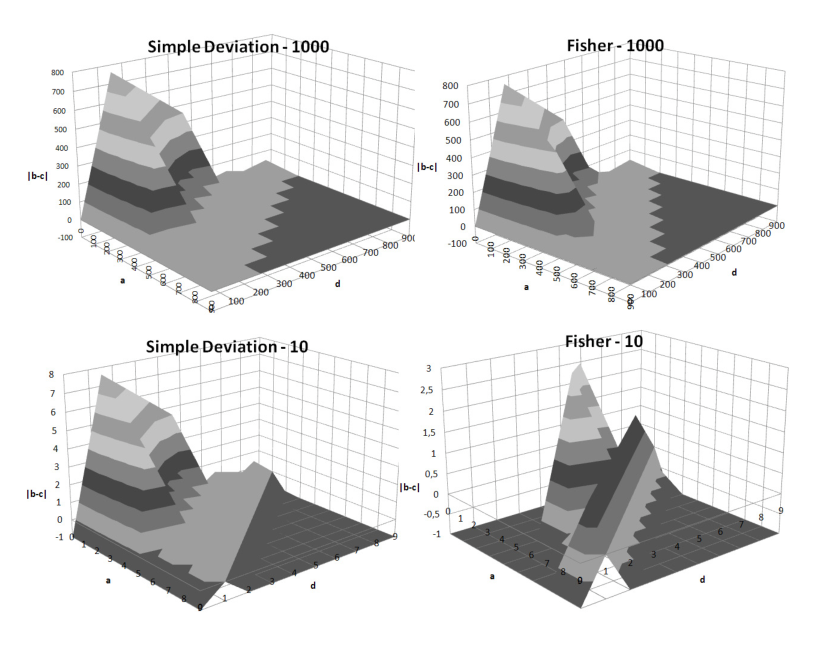
\includegraphics[width=115mm]{SDFisher.eps}
%\mbox{\resizebox{125mm}{!}{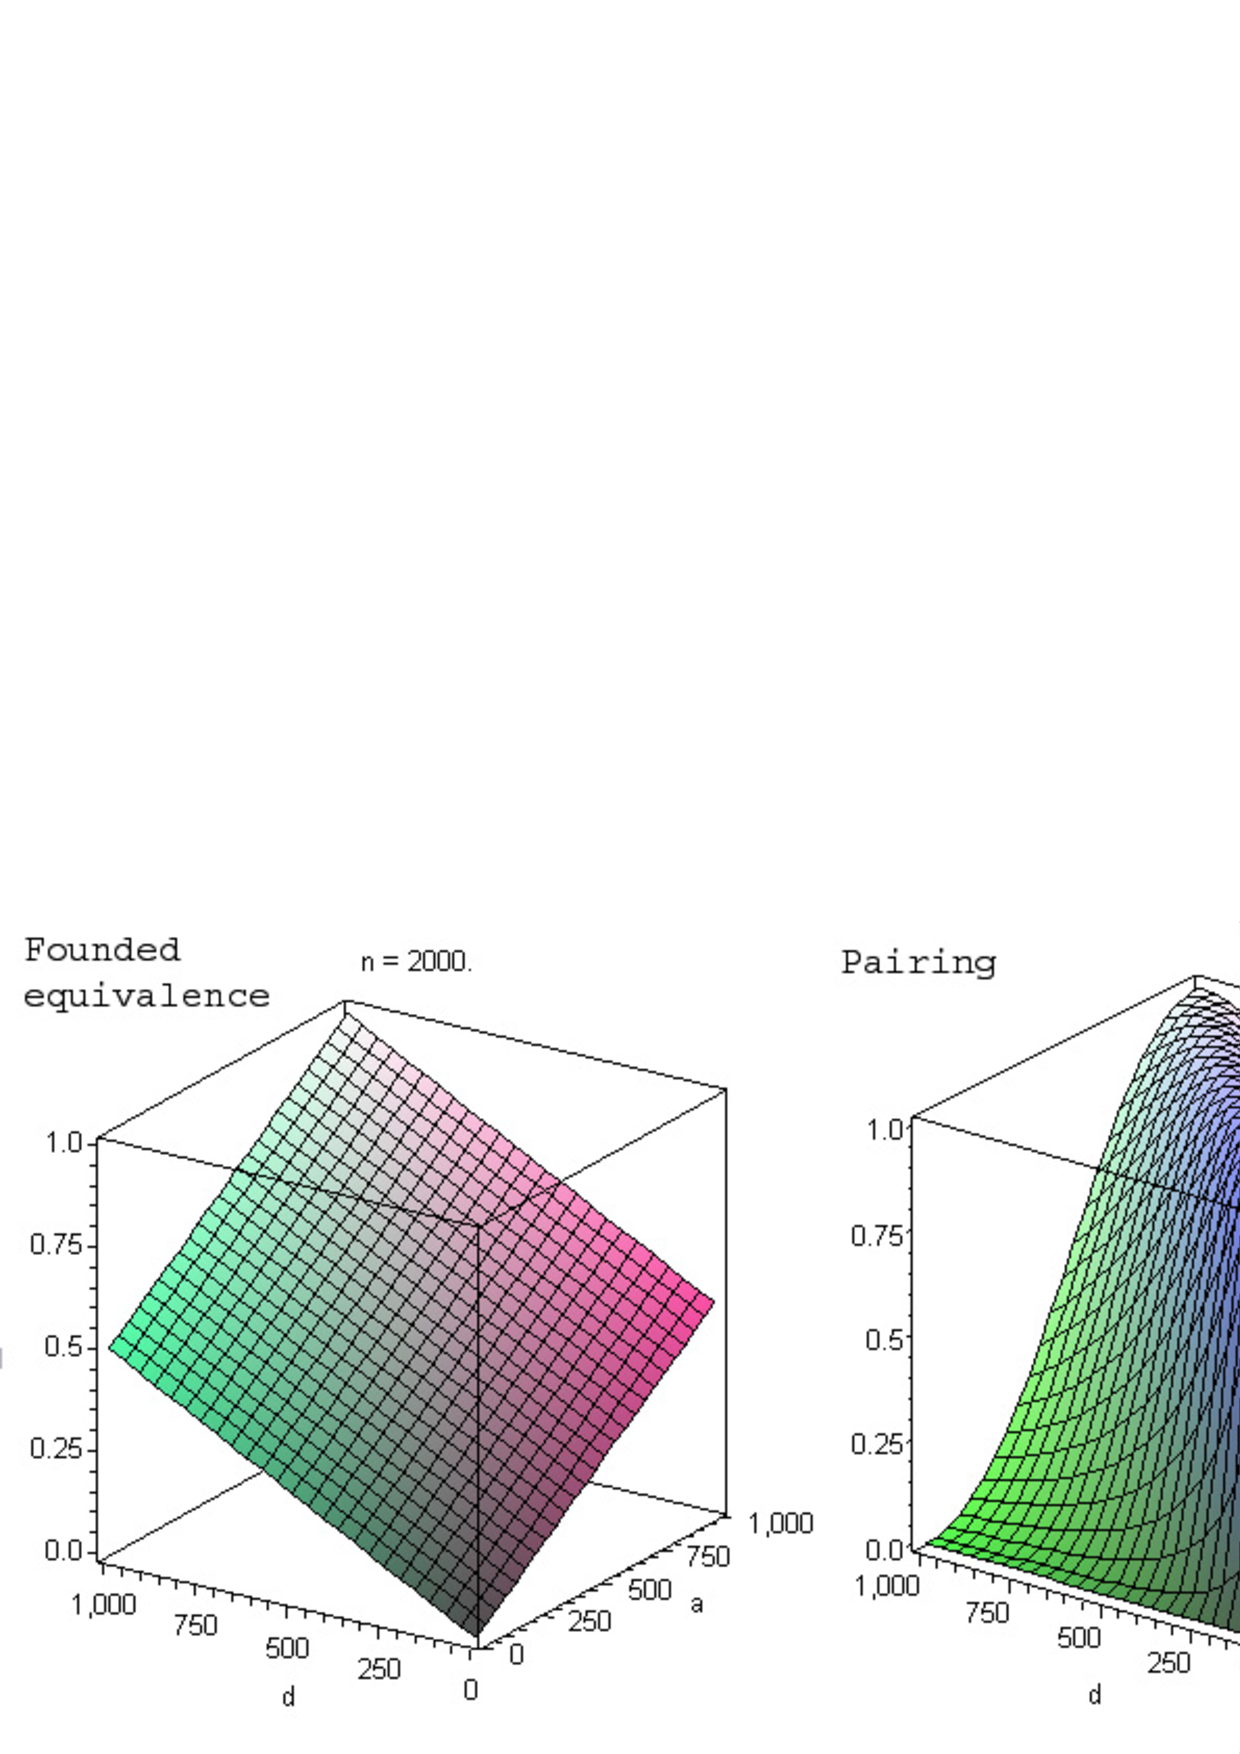
\includegraphics{FE-Pairing.png}}}
\caption{Tables of minimal $|b-c|$ for Fisher and Simple Deviation quantifiers}
\label{fig:FProperty}
\end{figure}

The graphs show, that \emph{Fisher's} quantifier behaves differently for $n=10$ and for $n=1000$. In the latter case, graphs of two quantifiers resemble each other, which was expcected. We did not compute values of the graph in all the possible points, we chose 100 representative points instead. Therefore the graphs only estimate real \emph{tables of minimal $|b-c|$}. For larger sizes of contingency tables, it is preferable to use the \emph{simple deviation}\footnote{Or $\chi^{2}$ quantifier, which was not introduced in this paper.}. 

We also examined the \emph{above average dependence} graph as shown in figure \ref{fig:AA}, with $n=1000$ and $p=0$ (this corresponds to $\delta=0$ for \emph{simple deviation}). Note, that all the graphs displayed have a similar feature: the quantifiers are \emph{F-strongest} along the inverse $ad$ diagonal. This is the most interesting result of experiments with tables of minimal $|b-c|$. It is a promising important characteristics of quantifiers with F-property, and should receive further attention. 

\begin{figure}[h]
\centering
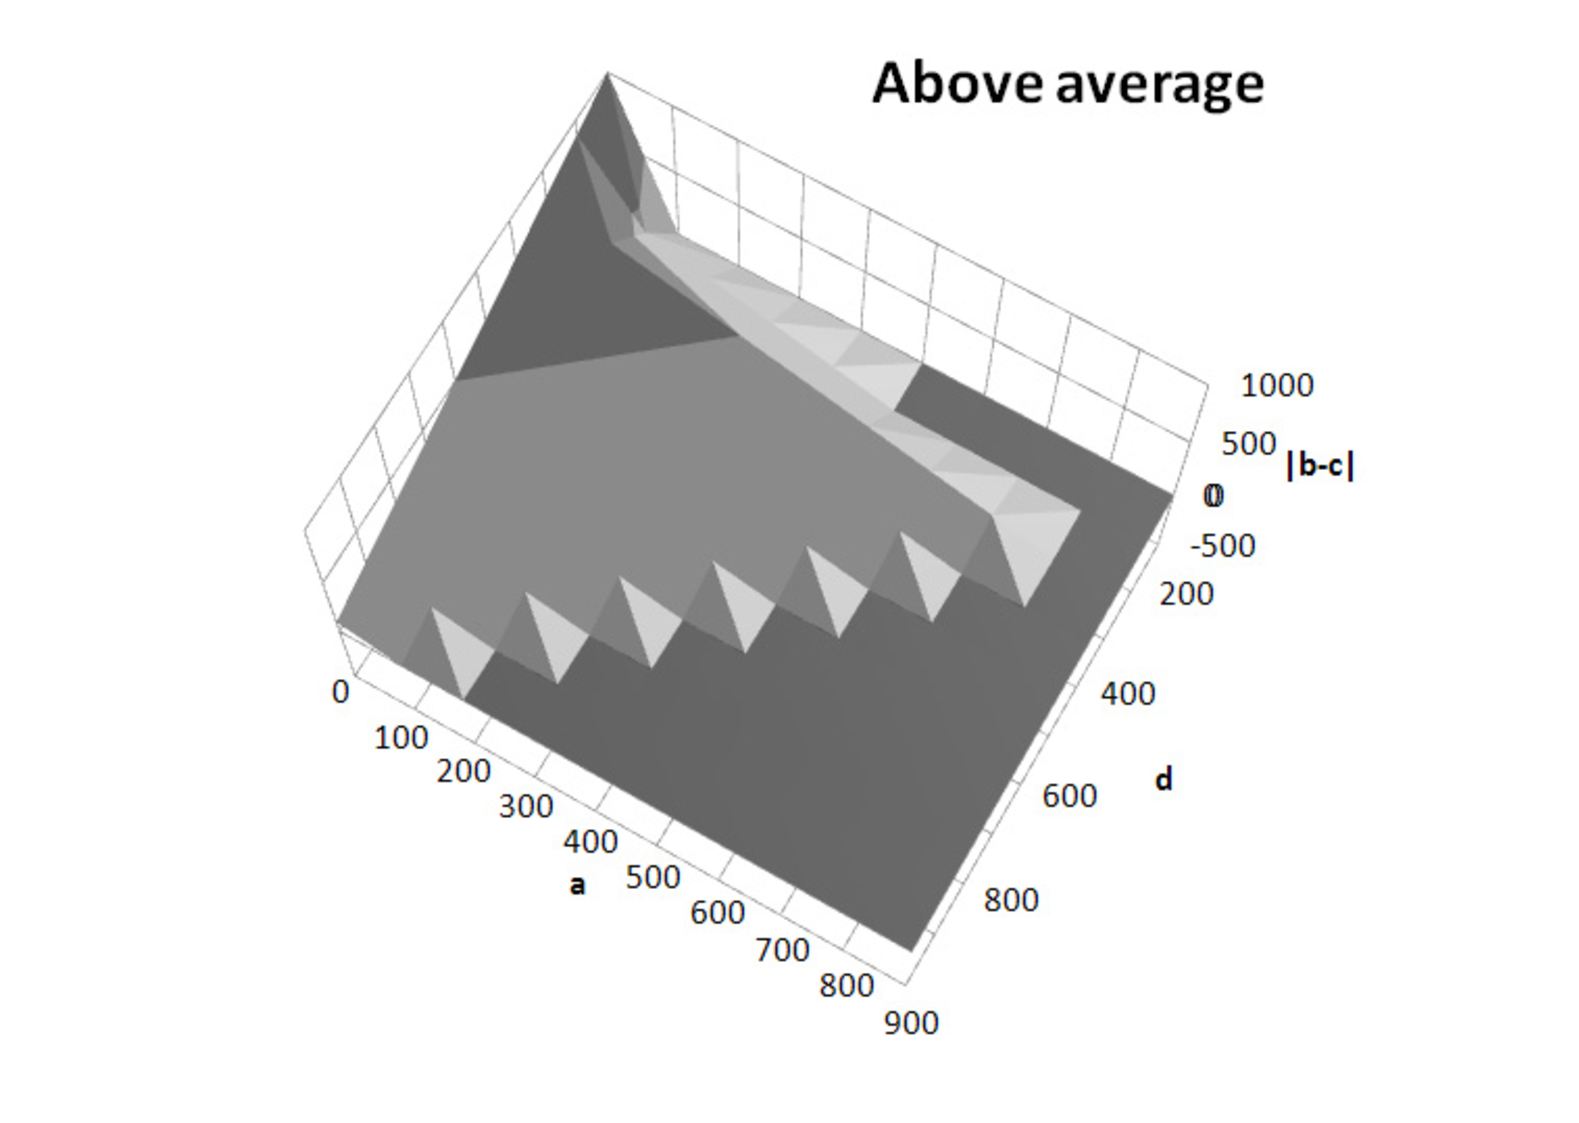
\includegraphics[width=70mm]{AA.eps}
%\mbox{\resizebox{125mm}{!}{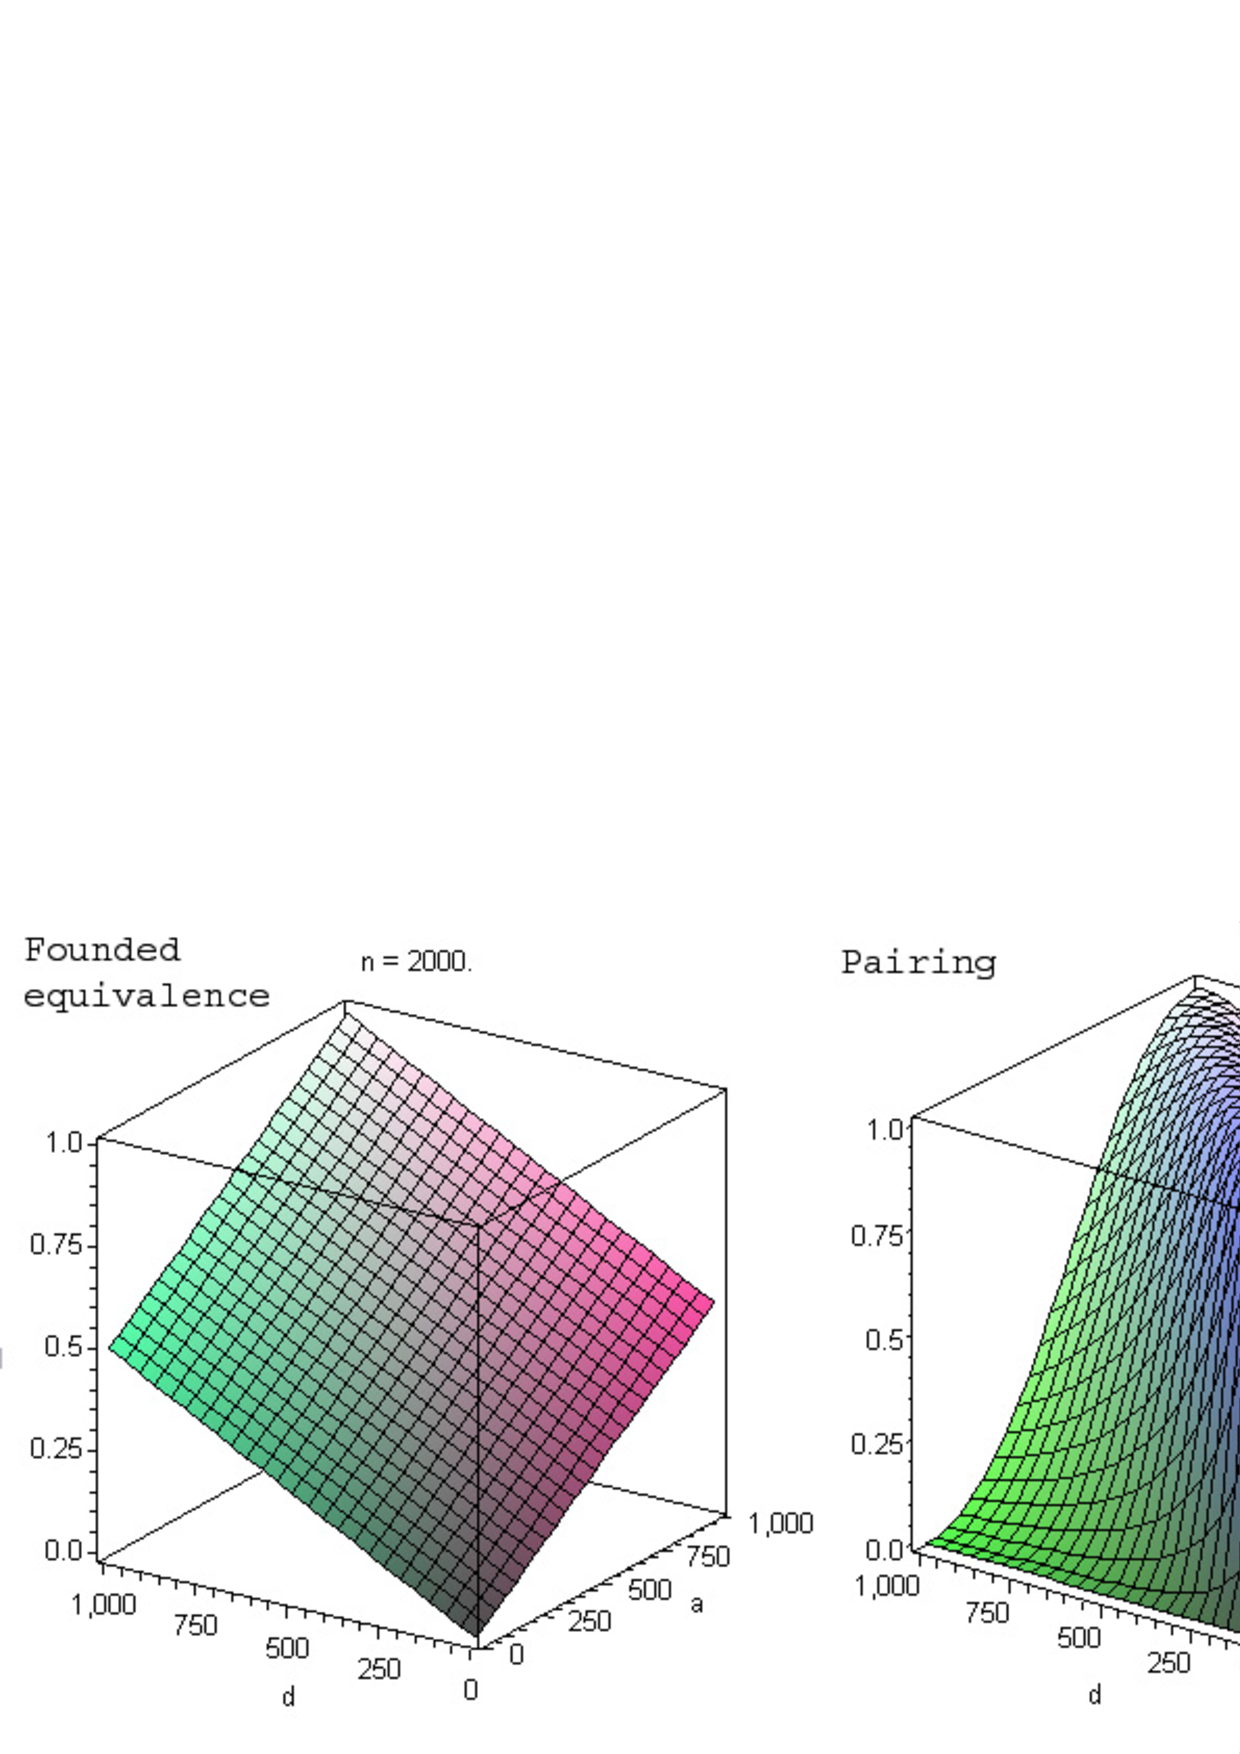
\includegraphics{FE-Pairing.png}}}
\caption{Tables of minimal $|b-c|$ for Above average dependence quantifier}
\label{fig:AA}
\end{figure}

The points along the inverse $ad$ diagonal have a common property, that is their sum is equal or close to $n$. This means that there is not much left for $b$ and $c$ (from $n$, the size of the contingency table). This explains, why values of minimal $|b-c|$ are so low along the inverse $ad$ diagonal, but it does not explain the fact, that the all three examined quantifiers are valid along this diagonal\footnote{This is rather obvious for \emph{simple deviation} quantifier, but not obvious for quantifiers with the F-property at all}. The validity of quantifiers with F-property along the inverse $ad$ diagonal remains an open question.